% Appendix D

\chapter{Labview: key functions} % Main appendix title
\label{AppendixE} % For referencing this appendix elsewhere, use \ref{AppendixA}
\lhead{Appendix D. \emph{Labview: key functions}} % This is for the header on each page - perhaps a shortened title

\section{Envelope program}

\begin{figure}[htbp]
\centering
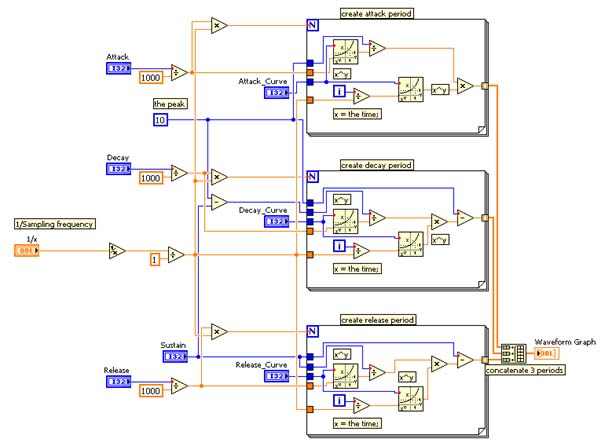
\includegraphics[height=12cm]{envprog}
\rule{30em}{0.5pt}
\caption{Envelope program}
%\label{fig:sharc}
\end{figure}
\newpage
\section{Clipping program}

\begin{figure}[!h]
\centering
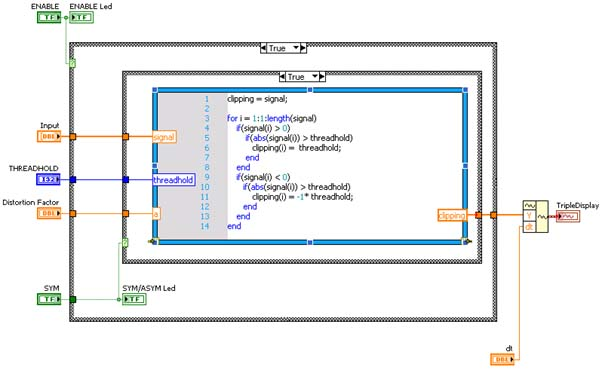
\includegraphics[height=8cm]{clipping}
\rule{30em}{0.5pt}
\caption{Clipping program}
%\label{fig:sharc}
\end{figure}

\section{Equaliser program}

\begin{figure}[!htbp]
\centering
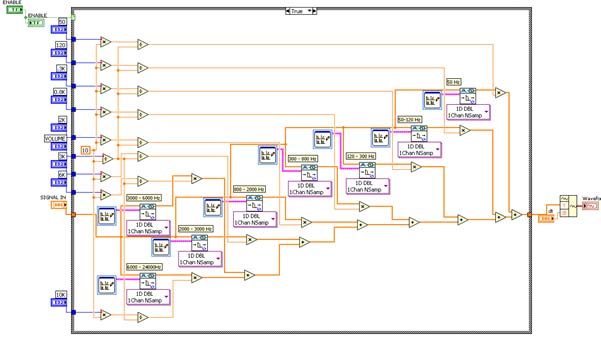
\includegraphics[height=9cm]{equaliser}
\rule{30em}{0.5pt}
\caption{Equaliser program}
%\label{fig:sharc}
\end{figure}
